\begin{figure*}[t]
  \centering
  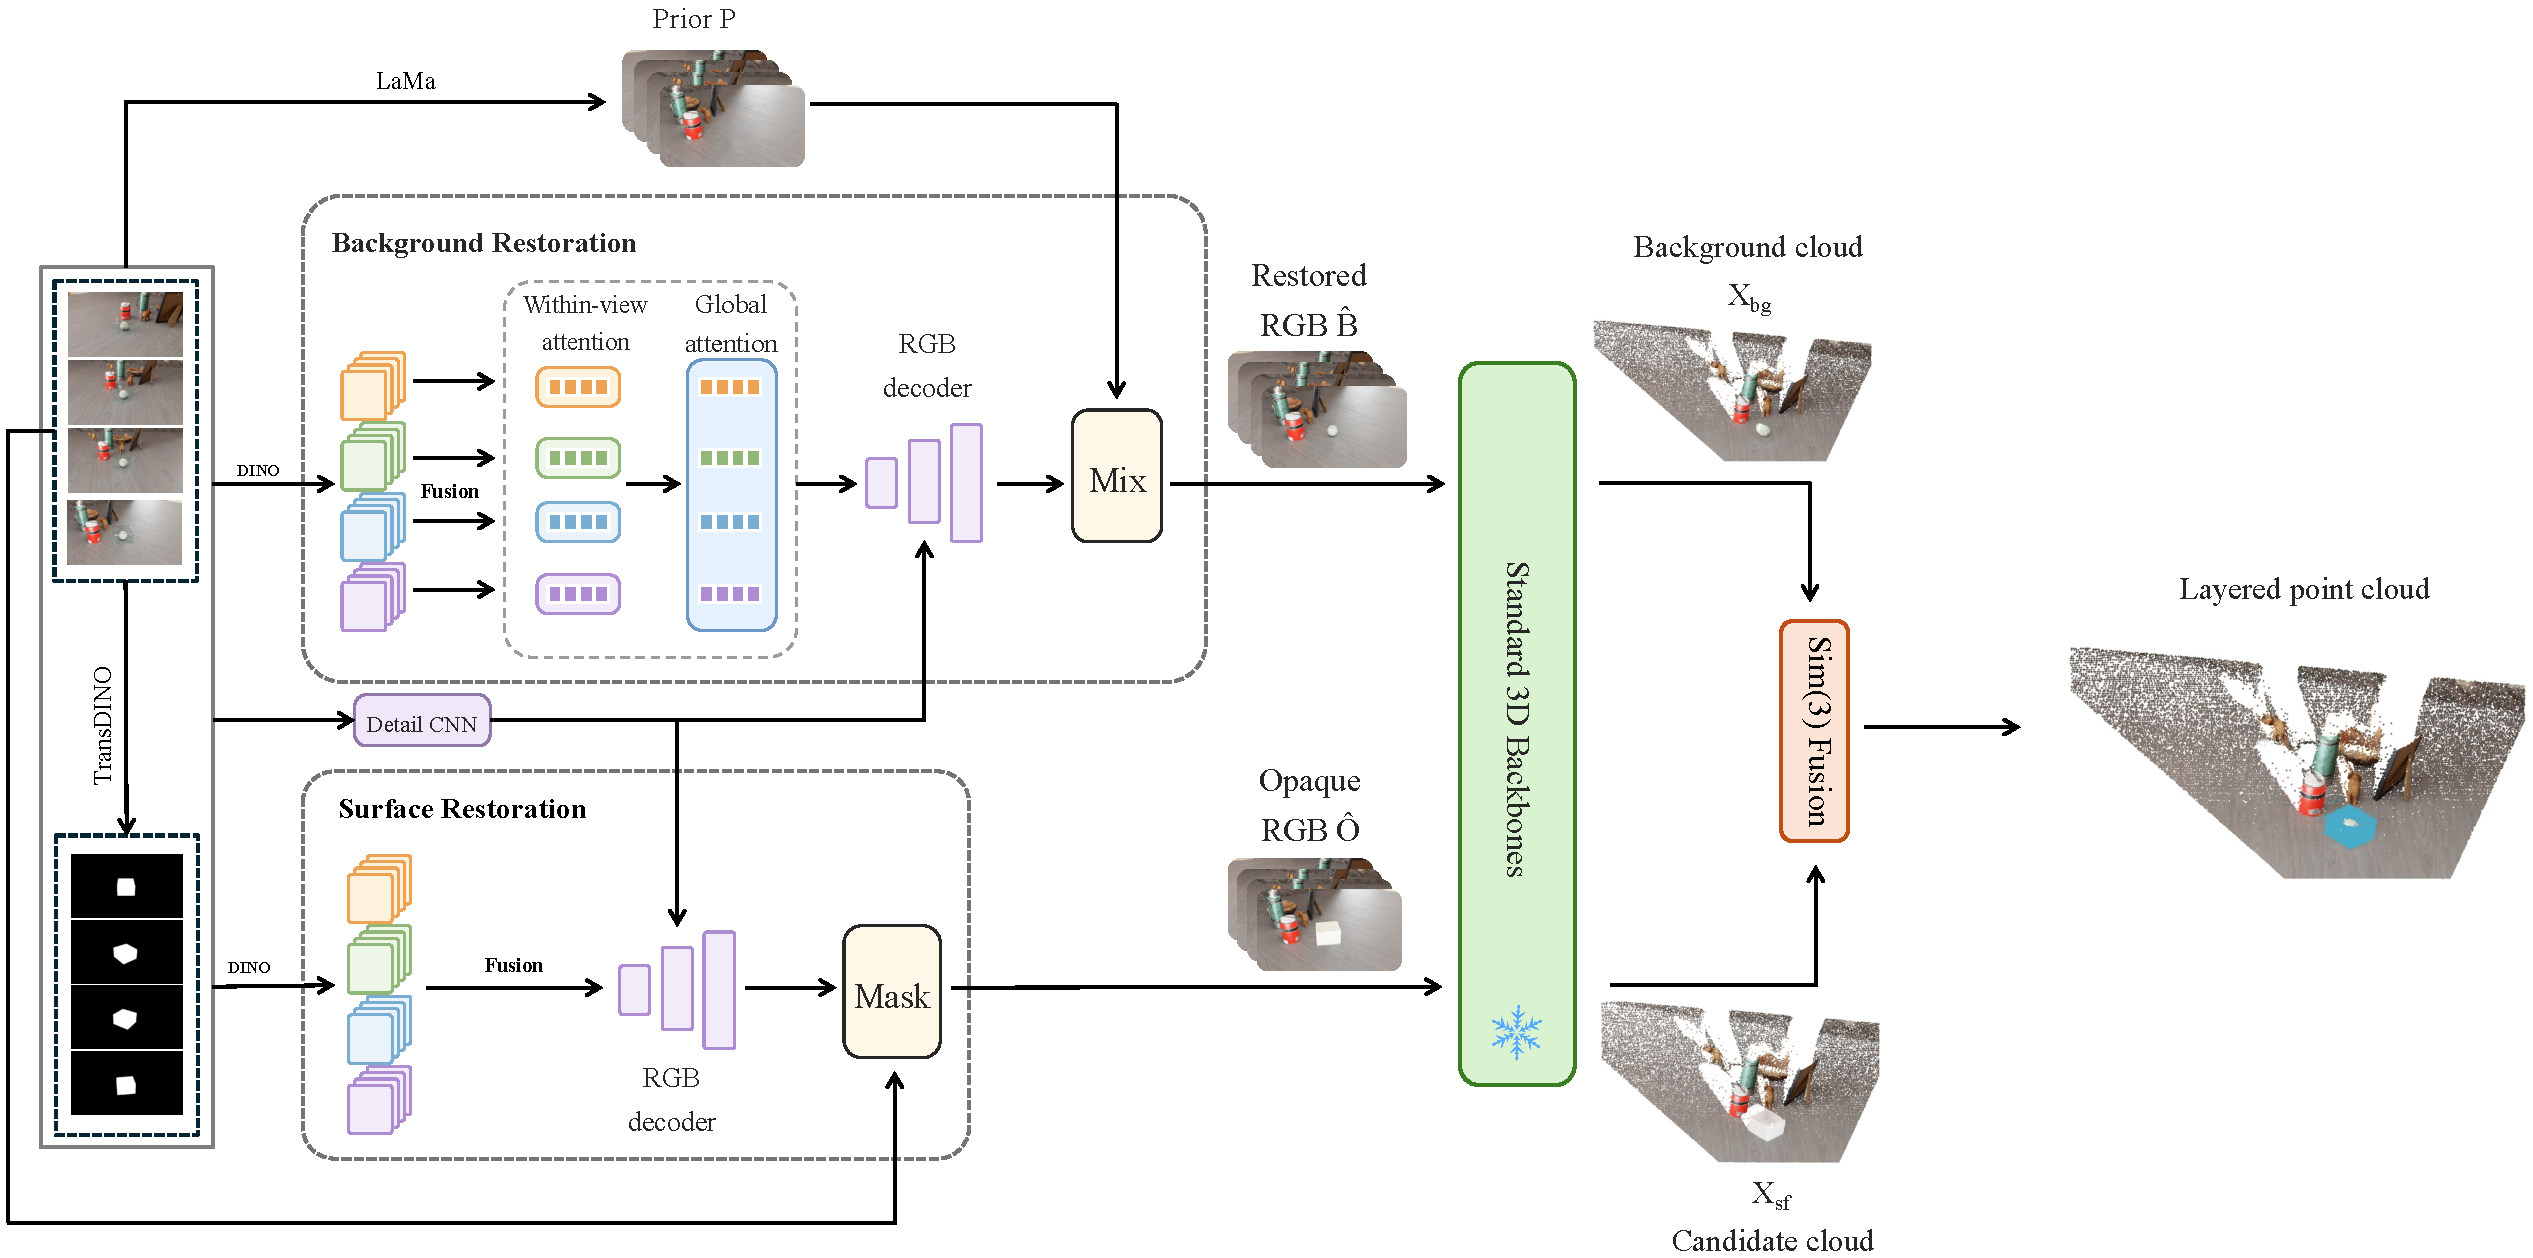
\includegraphics[width=\textwidth]{fig/method/output/architecture_slide3.pdf}
  \caption{\textbf{Overview of Phantom.}
  Given views $I$ and TransDINO masks $\hat M$~\cite{ghost}, the background front-end $\mathcal{F}_{bg}$ restores the scene behind the glass, $\hat B$, with attention across all views and a per-pixel mix with a LaMa prior $P$; the surface front-end $\mathcal{F}_{sf}$ renders the object opaque in each view, $\hat O$.
  A frozen geometry backbone $\mathcal{G}$ maps $\hat B$ and $\hat O$ to point clouds $X_{bg}$ and $X_{sf}$, which are aligned outside the mask and merged into a layered point cloud.}
  \label{fig:method}
\end{figure*}
